\section{Bài 2:}

Nhóm đóng vai trò là kỹ sư mạng của một công ty, nhóm được giao nhiệm vụ xây dựng hệ thống mạng cho văn phòng mới của công ty.

\bf Mô tả yêu cầu hệ thống:
\begin{enumerate}
\it\item Công ty sử dụng dãy địa chỉ 172.XX.0.0/16 để chia đường mạng cho toàn hệ thống để mỗi phòng/tầng/nhu cầu có đường mạng riêng.

\it\item Tòa nhà của công ty có 4 tầng:
\begin{enumerate}
\sc \item Tầng 1: \rm phòng hành chính (10 users), và một mạng wi-fi cho nhân viên và khách vãng lai (tối đa 20 users)

\sc \item Tầng 2: \rm phòng kỹ thuật (5 users), phòng lãnh đạo (tối đa 5 users)

\sc \item Tầng 3: \rm phòng họp dùng mạng wifi (tối đa 20 users)

\sc \item Tầng 4: \rm phòng server dùng địa chỉ IP tĩnh (tối đa 10 hosts)
\begin{enumerate}
\tt \item Dịch vụ DHCP: \rm triển khai trên 1 server duy nhất/ 1 router để cung cấp dải IP động cho các phòng ban ở tầng 1-2-3

\rm Gợi ý: cấu hình DHCP relay-agent bằng câu lệnh helper-address trên router

\tt \item Dịch vụ DNS phân giải tên miền: \rm mmt-XX.com

\tt \item Dịch vụ WEB \rm để người dùng có thể truy cập trang web công ty từ mạng nội bộ của công ty với tên miền: www.mmt-XX.com. Nội dung trang WEB: hiển thị thông tin MSSV - Họ tên thành viên của nhóm
\end{enumerate}

\sc \item Thiết bị mạng ở các phòng ban có thể kết nối lẫn nhau.
\end{enumerate}
\end{enumerate}

Yêu cầu:
\begin{enumerate}
\bf \item Phân tích hiện trạng và nhu cầu của công ty. Hãy vẽ sơ đồ mạng logic cho văn phòng công ty (có ghi chú tên thiết bị, tên interface/ port, IP, subnet).

\rm 

\bf \item Lập bảng mô tả chi tiết thiết bị gồm: khu vực đặt thiết bị, loại thiết bị, tên thiết bị, version/model, chức năng, tên interface/port, IP

\rm

\bf \item Sử dụng công cụ packet tracer để triển khai mô hình mạng đã thiết kế (chụp hình các bước triển khai cấu hình)

\rm

\bf \item Kiểm tra kết quả hoạt động của mô hình mạng vừa triển khai (dùng các câu lệnh console như ping, nslookup, ipconfig, và trình duyệt web)

\rm Lưu ý:
\begin{enumerate}
\item Chỉ sử dụng phương thức cấu hình định tuyến tĩnh

\item Chỉ sử dụng số lượng PC vừa đủ để kiểm tra hoạt động của mô hình, không cần thiết vẽ đầy đủ số host cho mỗi đường mạng trong mô hình

\item XX là 2 chữ số cuối của MSSV. Nếu làm nhóm 3 người, thì chọn MSSV của một trong 3 bạn.
\end{enumerate}

\end{enumerate}

Trả lời:

\begin{enumerate}
\bf \item Phân tích hiện trạng và nhu cầu của công ty. Hãy vẽ sơ đồ mạng logic cho văn phòng công ty (có ghi chú tên thiết bị, tên interface/ port, IP, subnet).

\rm \textbf{Hiện trạng và nhu cầu của công ty:} Công ty đã có dãy địa chỉ \textcolor{red}{\bf 172.72.0.0/16} cần chia cho toàn hệ thống (dùng số lượng host tối đa theo yêu cầu):

\begin{enumerate}
\item Tầng 1: 

\(\bullet\) 1 đường mạng cho phòng hành chính - 10 users

\(\bullet\) 1 đường mạng wi-fi cho nhân viên + khách vãng lai - 20 users

\item Tầng 2:

\(\bullet\) 1 đường mạng cho phòng kỹ thuật - 5 users

\(\bullet\) 1 đường mạng cho phòng lãnh đạo - 5 users

\item Tầng 3:

\(\bullet\) 1 đường mạng wi-fi cho phòng họp - 20 users

\item Tầng 4:

\(\bullet\) 1 đường mạng - 10 servers.

\end{enumerate}

\textbf{Ta thực hiện chia subnet như sau:}

\it Có tổng cộng 6 subnets, trong đó subnet cần nhiều hosts/users nhất là 20 \(\Rightarrow\) cần giữ lại \(m\) bit host sao cho \(2^m-2\ge 20\Rightarrow m\ge 5\), do đó ta được mượn tối đa \(32-16-5 = 11\) bit net. 

Mà ta chỉ cần 6 subnets do đó ta chỉ cần mượn 3 bit (ở byte 3), chia được thành 8 địa chỉ đường mạng con (subnet), mỗi subnet này cho phép số địa chỉ host hợp lệ là \(2^{32-16-3}-2 = 8190 > 20\).
\begin{table}[H]
\begin{center}
\begin{tabular}{|c|c|c|c|c|}
\hline
STT & Đ/c đường mạng & Subnet mask & Đ/c broadcast & Dải đ/c host hợp lệ\\
\hline
1 & 172.72.0.0 & 255.255.224.0 & 172.72.31.255 & 172.72.0.1 - 172.72.31.254\\
\hline
2 & 172.72.32.0 & 255.255.224.0 & 172.72.63.255 & 172.72.32.1 - 172.72.63.254\\
\hline
3 & 172.72.64.0 & 255.255.224.0 & 172.72.95.255 & 172.72.64.1 - 172.72.95.254\\
\hline
4 & 172.72.96.0 & 255.255.224.0 & 172.72.127.255 & 172.72.96.1 - 172.72.127.254\\
\hline
5 & 172.72.128.0 & 255.255.224.0 & 172.72.159.255 & 172.72.128.1 - 172.72.159.254\\
\hline
6 & 172.72.160.0 & 255.255.224.0 & 172.72.191.255 & 172.72.160.1 - 172.72.191.254\\
\hline
7 & 172.72.192.0 & 255.255.224.0 & 172.72.223.255 & 172.72.192.1 - 172.72.223.254\\
\hline
8 & 172.72.224.0 & 255.255.224.0 & 172.72.255.255 & 172.72.224.1 - 172.72.255.254\\
\hline
\end{tabular}
\caption{Chia subnet}
\end{center}
\end{table}

Sau đó ta chia cho mỗi nhu cầu/phòng ban một đường mạng con/subnet như sau:
\rm
Subnet 172.72.0.0/19 dùng cho phòng hành chính, tầng 1 (10 hosts).

Subnet 172.72.32.0/19 dùng cho mạng wi-fi nhân viên và khách vãng lai, tầng 1 (20 hosts).

Subnet 172.72.64.0/19 dùng cho phòng kỹ thuật, tầng 2 (5 hosts).

Subnet 172.72.96.0/19 dùng cho phòng lãnh đạo, tầng 2 (5 hosts).

Subnet 172.72.128.0/19 dùng cho mạng wi-fi phòng họp, tầng 3 (20 hosts).

Và lấy 10 địa chỉ IP tĩnh trong subnet 172.72.160.0/19 để cấp cho 10 servers, cụ thể ta sẽ chọn dãy địa chỉ 172.72.160.1 - 172.72.160.10 để cấp, trong đó
\begin{enumerate}
\item Dịch vụ DHCP: triển khai trên server 172.72.160.1

\item Dịch vụ DNS: triển khai trên server 172.72.160.2

\item Dịch vụ WEB: triển khai trên server 172.72.160.3
\end{enumerate}

\textbf{Sơ đồ mạng logic cho văn phòng công ty được thiết kế như sau:}

\begin{figure}[H]
\begin{center}
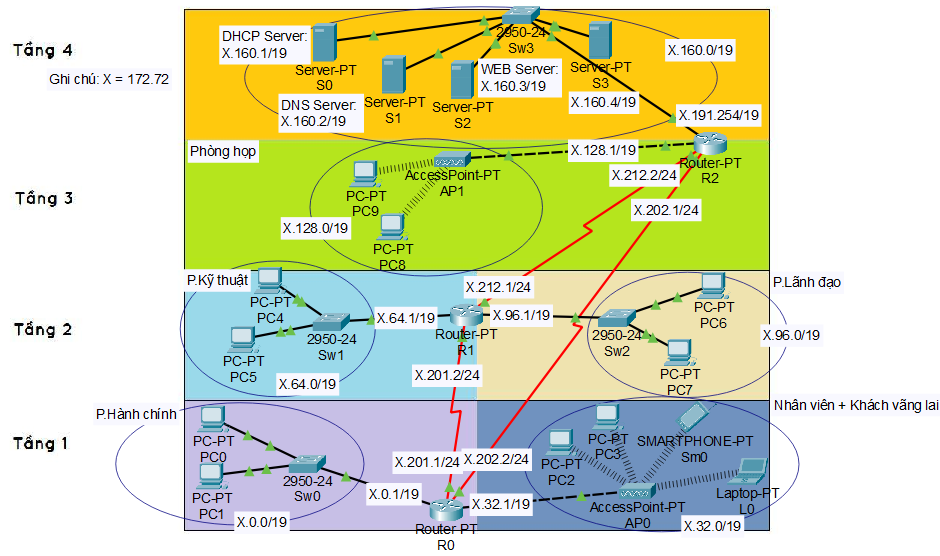
\includegraphics[scale=.9]{../figures/p2/sodo}
\end{center}
\caption{Sơ đồ mạng logic cho văn phòng công ty}
\end{figure}

\bf \item Lập bảng mô tả chi tiết thiết bị gồm: khu vực đặt thiết bị, loại thiết bị, tên thiết bị, version/model, chức năng, tên interface/port, IP

\rm
\begin{longtable}{|p{1cm}|p{6cm}|p{4cm}|c|}
\hline
Tên thiết bị & \multicolumn{1}{c|}{Chức năng - Khu vực} & \multicolumn{1}{c|}{Interface/Port} & IP\\
\hline
\multicolumn{4}{|p{\linewidth}|}{Các Router [Router-PT]: Kết nối các mạng logic khác nhau, sử dụng địa chỉ IP để xử lý gói tin, định tuyến và chuyển tiếp gói tin. Số lượng: 3}\\
\hline
\multirow{4}*{R0} & \multirow{4}{=}{Kết nối giữa 2 đường mạng ở tầng 1 và 2 router R1, R2} & FastEthernet0/0 & 172.72.0.1/19 \\
 & & FastEthernet1/0 & 172.72.32.1/19 \\
 & & Serial2/0 & 172.72.201.1/24\\
 & & Serial3/0 & 172.72.202.2/24\\
\hline
\multirow{4}*{R1} & \multirow{4}{=}{Kết nối giữa 2 đường mạng ở tầng 2 và 2 router R0, R2} & FastEthernet0/0 & 172.72.64.1/19 \\
 & & FastEthernet1/0 & 172.72.96.1/19 \\
 & & Serial2/0 & 172.72.212.1/24\\
 & & Serial3/0 & 172.72.201.2/24\\
\hline
\multirow{4}*{R2} & \multirow{4}{=}{Kết nối giữa 2 đường mạng ở tầng 3, 4 và 2 router R0, R1} & FastEthernet0/0 & 172.72.128.1/19 \\
 & & FastEthernet1/0 & 172.72.191.254/19 \\
 & & Serial2/0 & 172.72.202.1/24\\
 & & Serial3/0 & 172.72.212.2/24\\
\hline
\multicolumn{4}{|p{\linewidth}|}{Các Switch [2950-24] (gồm 24 port): Kết nối 2 nhánh mạng vật lý, chuyển tiếp gói tin có chọn lọc (filtering/forwarding), duy trì bảng địa chỉ MAC. Số lượng: 4}\\
\hline
Sw0 & Phòng hành chính (10 máy) & FastEthernet0/1-24 & - \\
\hline
Sw1 & Phòng kỹ thuật (5 máy) & FastEthernet0/1-24 & - \\
\hline
Sw2 & Phòng lãnh đạo (5 máy) & FastEthernet0/1-24 & - \\
\hline
Sw3 & Tầng 4 (10 máy) & FastEthernet0/1-24 & - \\
\hline
\multicolumn{4}{|p{\linewidth}|}{Các Access Point [AccessPoint-PT]: Cho phép các thiết bị truy cập mạng không dây. Số lượng: 2}\\
\hline
AP0 & Nhân viên + Khách vãng lai (20 thiết bị) & Port0: Nối với router R0; Port1: SSID: wifi-tang-1, Authentication: WPA2-PSK, Pass phrase: 172-72-32 & -\\
\hline
AP1 & Phòng họp (20 thiết bị) & Port0: Nối với router R0; Port1: SSID: wifi-tang-3, Authentication: WPA2-PSK, Pass phrase: 172-72-128 & -\\
\hline
\multicolumn{4}{|p{\linewidth}|}{Các Server [Server-PT]. Số lượng: 10, thể hiện 4 servers: 3 servers cho 3 yêu cầu + 1 server đại diện cho 7 server còn lại}\\
\hline
S0 & DHCP Server: Cấp phát địa chỉ IP động cho các hosts & FastEthernet0 & 172.72.160.1/19\\
\hline
S1 & DNS Server: Phân giải tên miền quản lý: mmt-72.com & FastEthernet0 & 172.72.160.2/19\\
\hline
S2 & WEB Server: Host của tên miền www.mmt-72.com & FastEthernet0 & 172.72.160.3/19\\
\hline
 & 7 server khác (đại diện là S3 với đ/c IP: 172.72.160.4/19) & FastEthernet0 & 172.72.160.(4-10)/19\\
\hline
\multicolumn{4}{|p{\linewidth}|}{Các PC [PC-PT]. Số lượng: 20 (10 + 5 + 5), có thể thêm ở các mạng wi-fi ở tầng 1 hoặc tầng 3, trong đó thể hiện 6 PC + một số PC có thể kết nối vào các mạng wi-fi vừa nói.}\\
\hline
 & Phòng hành chính (đại diện là PC0, PC1) & FastEthernet0 & [DHCP] 172.72.(0.2-31.254)/19\\
\hline
 & Phòng kỹ thuật (đại diện là PC4, PC5) & FastEthernet0 & [DHCP] 172.72.(64.2-95.254)/19\\
\hline
 & Phòng lãnh đạo (đại diện là PC6, PC7) & FastEthernet0 & [DHCP] 172.72.(96.2-127.254)/19\\
\hline
 & Nhân viên + khách vãng lai (nếu có, đại diện là PC2, PC3) & Wireless0 (SSID wifi-tang-1) & [DHCP] 172.72.(32.2-63.254)/19\\
\hline
 & Phòng họp (nếu có, đại diện là PC8, PC9) & Wireless0 (SSID wifi-tang-3) & [DHCP] 172.72.(128.2-159.254)/19\\
\hline
\multicolumn{4}{|p{\linewidth}|}{Các thiết bị End Devices khác, nếu có.}\\
\hline
 & Nhân viên + khách vãng lai (nếu có, đại diện là Smartphone Sm0, Laptop L0) & Wireless0 (SSID wifi-tang-1) & [DHCP] 172.72.(32.2-63.254)/19\\
\hline
 & Phòng họp (nếu có) & Wireless0 (SSID wifi-tang-3) & [DHCP] 172.72.(128.2-159.254)/19\\
\hline
\caption{Bảng mô tả chi tiết thiết bị}
\end{longtable}

\bf \item Sử dụng công cụ packet tracer để triển khai mô hình mạng đã thiết kế (chụp hình các bước triển khai cấu hình)

\rm 
\begin{enumerate}
\item Dịch vụ DHCP:

Mở Server \textsc{S0}, vào tab \textsc{Services}, chọn thẻ \textsc{DHCP}, sau đó bật Service thành On, cũng như điền thông tin tương ứng để cung cấp dải IP động cho các phòng ban từ tầng 1 đến tầng 3.

\begin{figure}[H]
\begin{center}
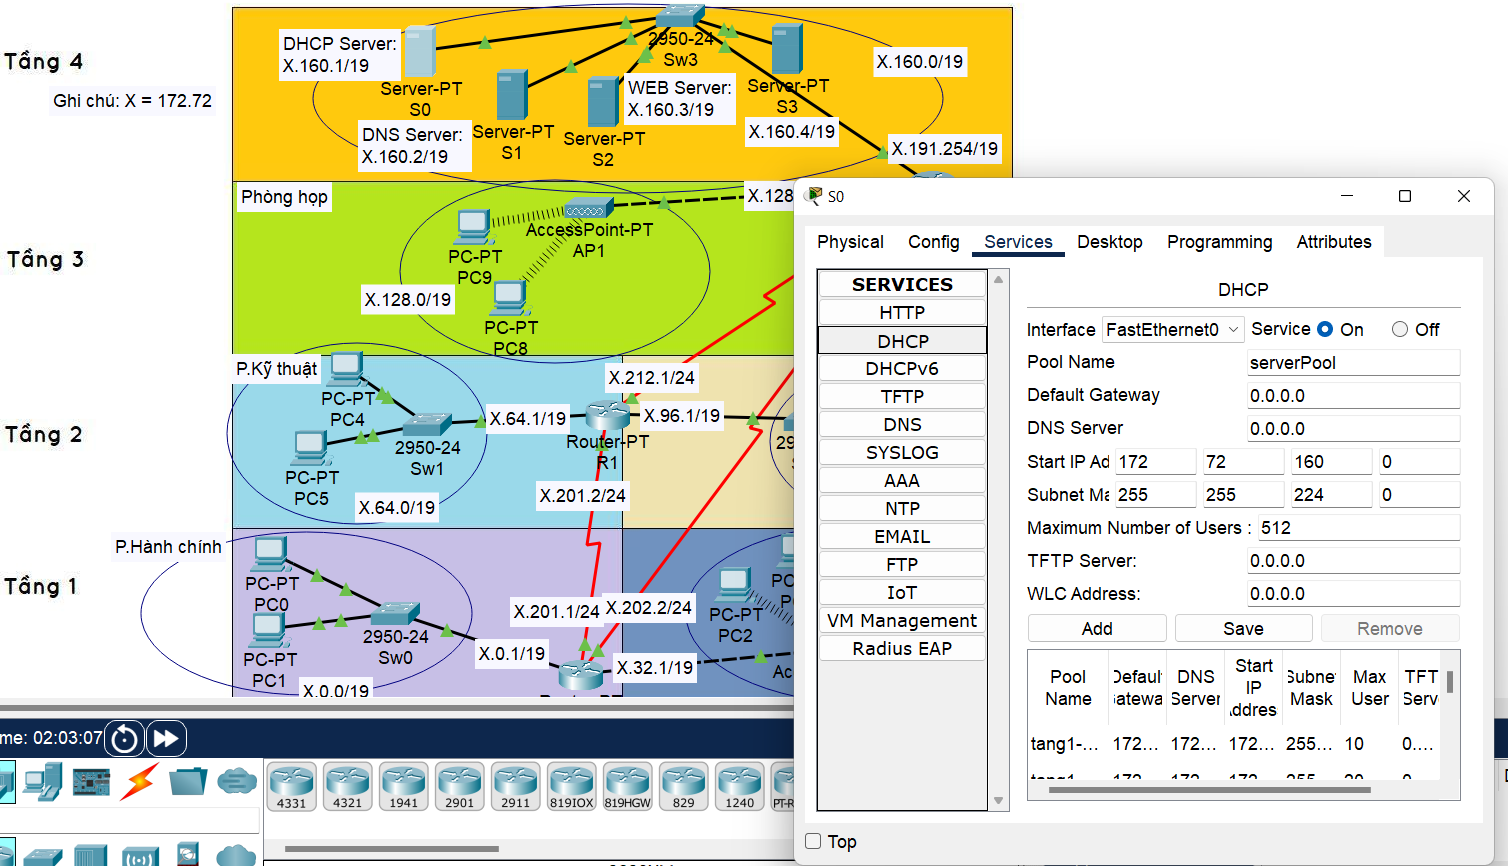
\includegraphics[scale=.5]{../figures/p2/dhcp1}
\end{center}
\caption{Triển khai dịch vụ DHCP trên server S0}
\end{figure}

Ví dụ sau đây là các thông tin để cung cấp IP động cho đường mạng phòng hành chính, tầng 1. Sau khi điền đầy đủ các thông tin, click Add để thêm vào bảng. Thực hiện tương tự cho wifi nhân viên + khách (tầng 1), phòng kỹ thuật (tầng 2), phòng lãnh đạo (tầng 2), wifi phòng họp (tầng 3). 
\begin{figure}[H]
\begin{center}
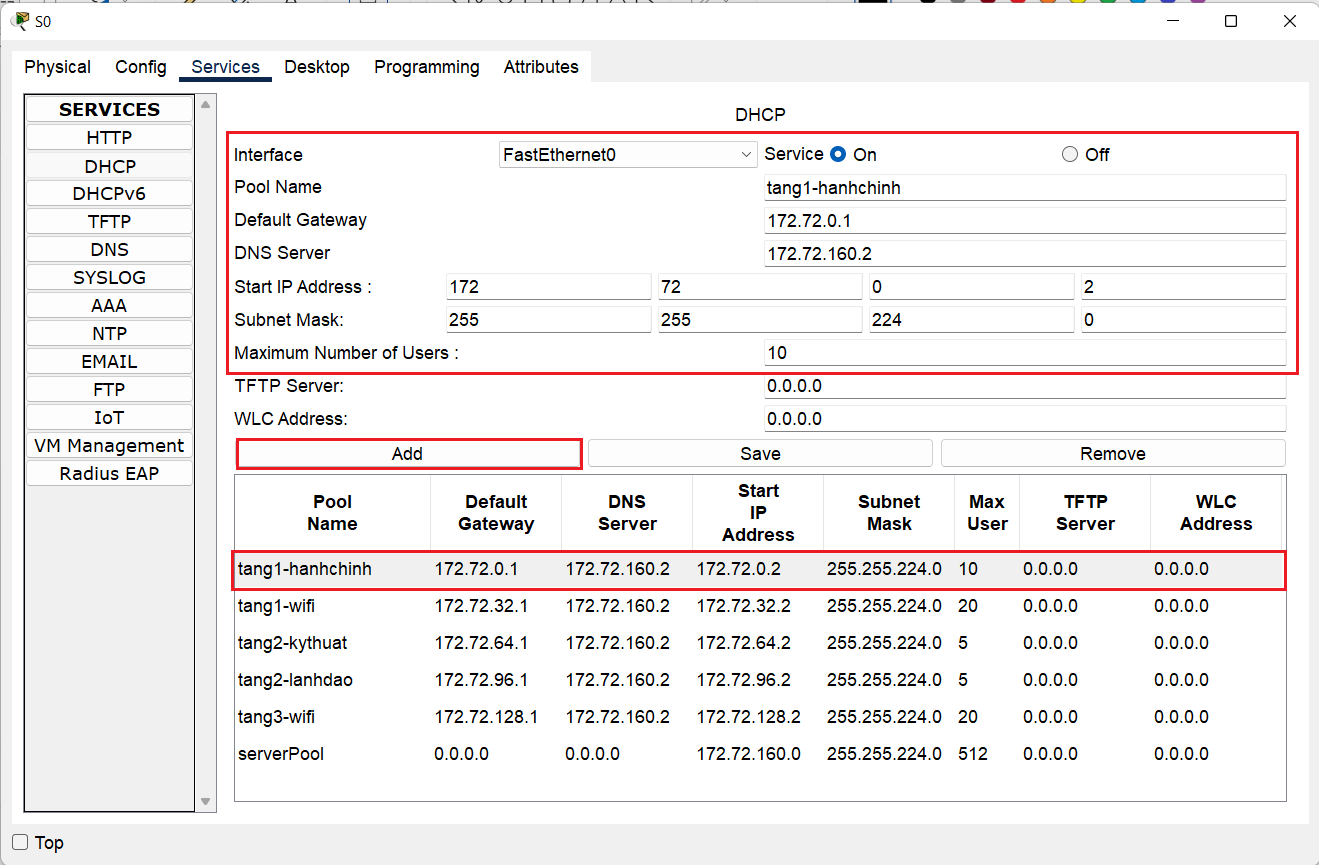
\includegraphics[scale=.7]{../figures/p2/dhcp2}
\end{center}
\caption{Điền các thông tin để cấp IP động cho mạng phòng hành chính, tầng 1}
\end{figure}

Về phía các hosts (PCs/các End Devices khác) sử dụng DHCP để cấp IP động, vào tab \textsc{Config}, sau đó vào tab \textsc{Global/Settings} và chọn DHCP ở phần Gateway/DNS IPv4 (hình vẽ minh họa cho các thiết bị Laptop L0, Smartphone Sm0, PC5)
\begin{figure}[H]
\begin{center}
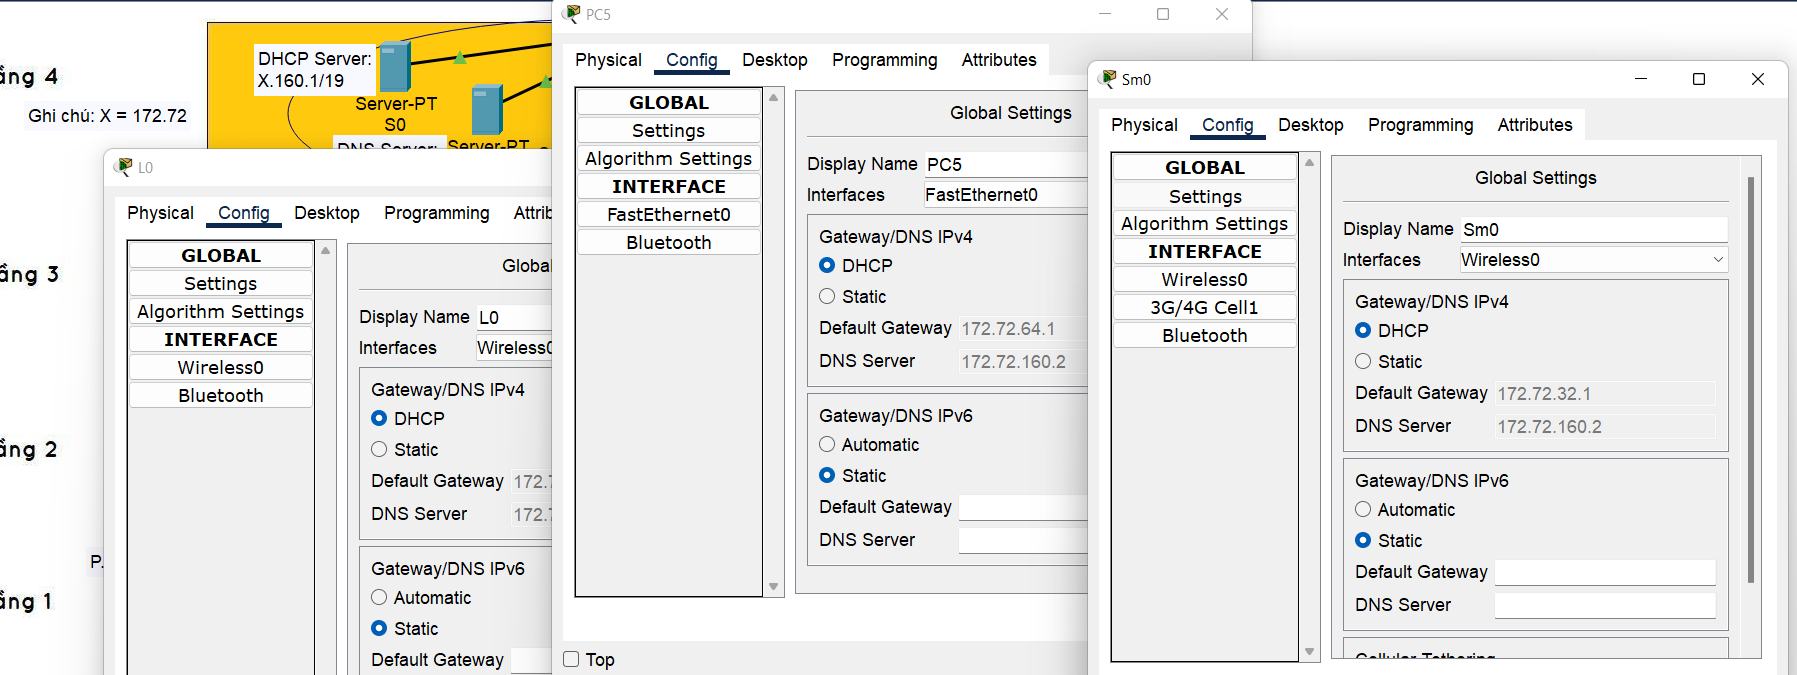
\includegraphics[scale=.5]{../figures/p2/dhcp3}
\end{center}
\caption{Cấu hình DHCP cho các hosts truy cập}
\end{figure}

\item Dịch vụ DNS: 

Mở Server \textsc{S1}, vào tab \textsc{Services}, chọn thẻ \textsc{DNS}, sau đó bật DNS Service thành On, sau đó nhập tên miền cần quản lý, chọn Type là \texttt{\textcolor{blue}{A Record}}, và địa chỉ IP tương ứng. Sau đó click Add để thêm vào bảng.

\begin{figure}[H]
\begin{center}
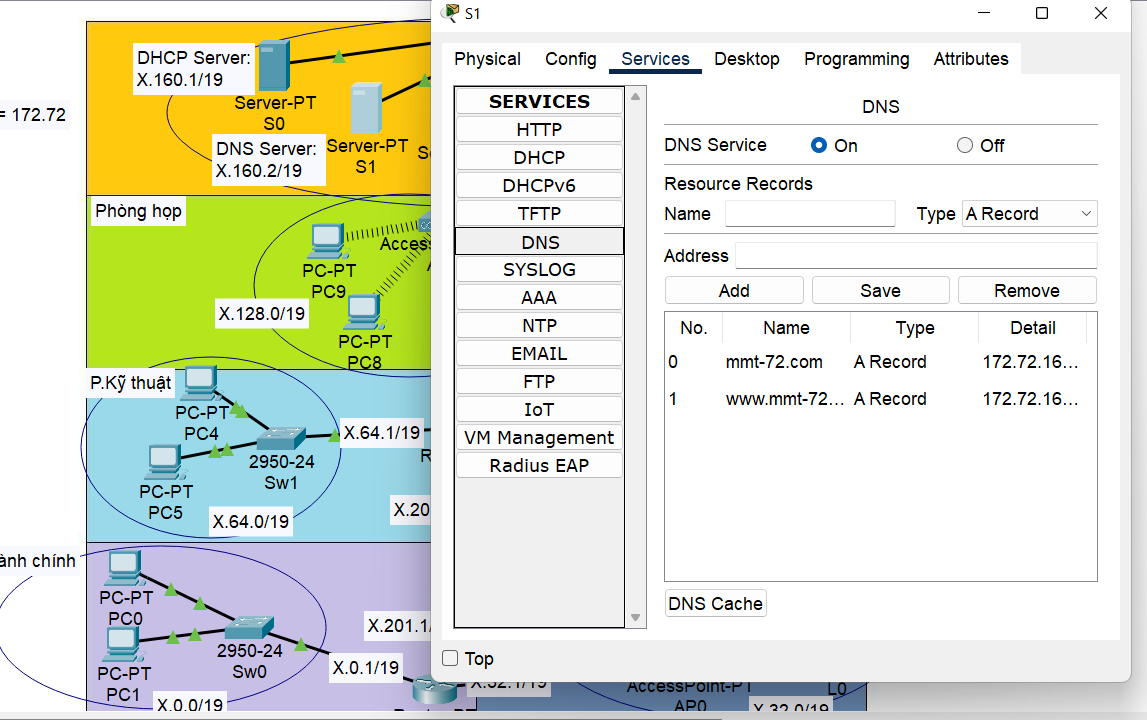
\includegraphics[scale=.5]{../figures/p2/dns1}
\end{center}
\caption{Triển khai dịch vụ DNS trên server S1}
\end{figure}

Hình vẽ dưới đây là các thông tin ứng với domain name \texttt{\textcolor{blue}{mmt-72.com}} ứng với địa chỉ IP của DNS server này, là \texttt{\textcolor{blue}{172.72.160.2}}.
\begin{figure}[H]
\begin{center}
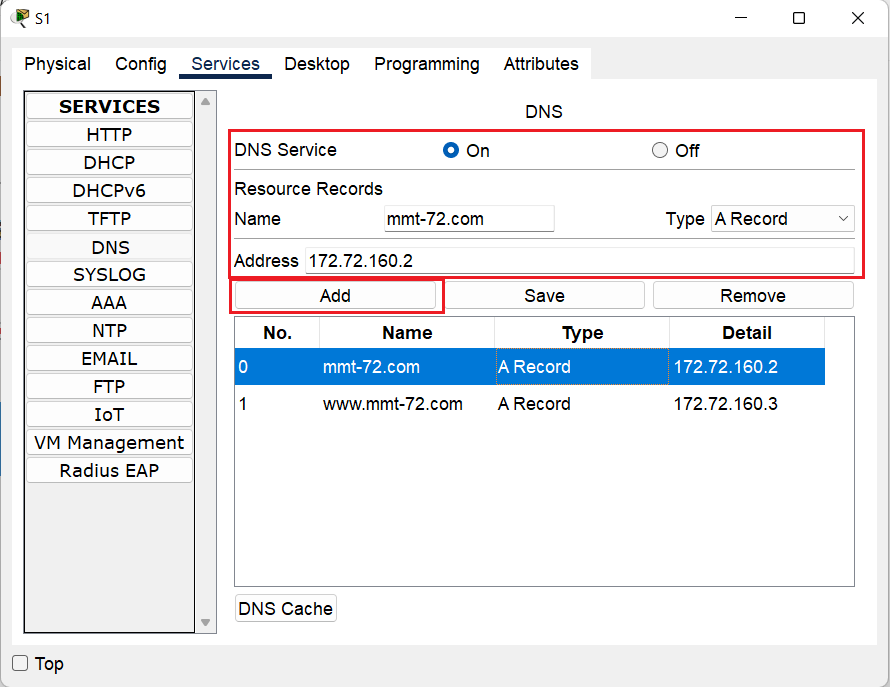
\includegraphics[scale=.7]{../figures/p2/dns2}
\end{center}
\caption{Điền các thông tin cho bản record domain name để DNS Server quản lý}
\end{figure}

Ta cũng thêm một bản record cho \texttt{\textcolor{blue}{www.mmt-72.com}} với địa chỉ IP \texttt{\textcolor{blue}{172.72.160.3}}.

\item Dịch vụ WEB:

Mở Server \textsc{S2}, vào tab \textsc{Services}, chọn thẻ \textsc{HTTP}, bật các options ở cả HTTP và HTTPS thành On, cũng như thực hiện thêm hoặc xóa các file \texttt{.html} tại đây.

\begin{figure}[H]
\begin{center}
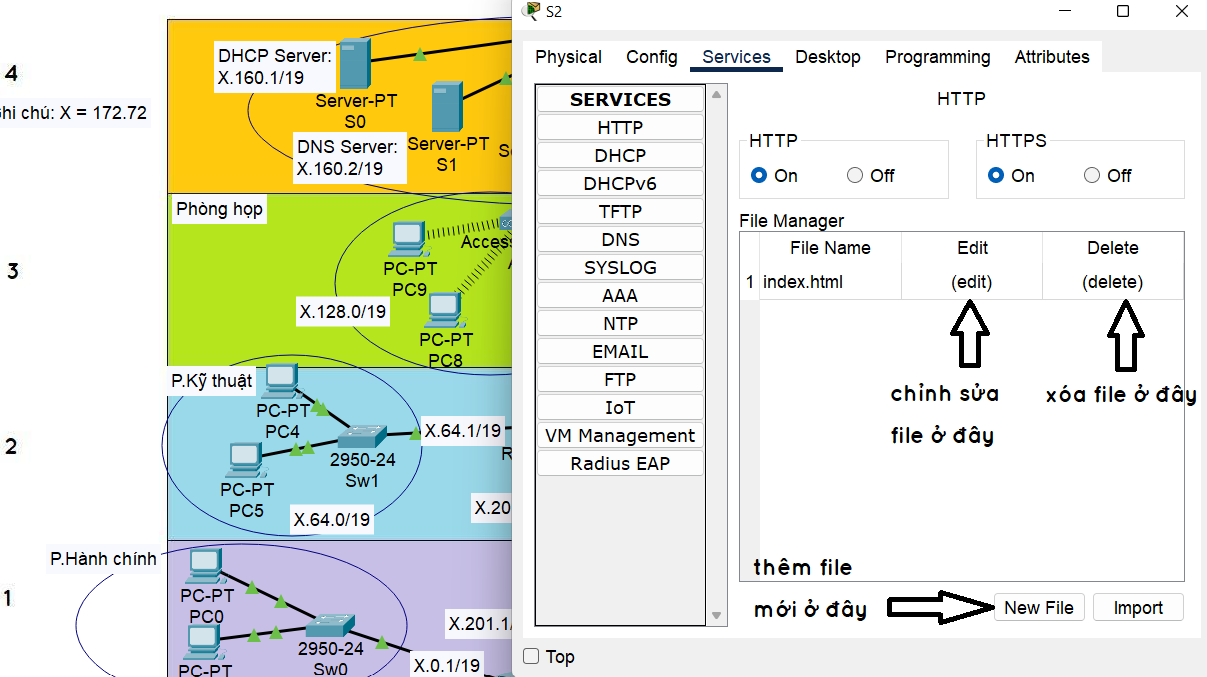
\includegraphics[scale=.5]{../figures/p2/web1}
\end{center}
\caption{Triển khai dịch vụ WEB trên server S2}
\end{figure}

Ta cũng có thể chỉnh sửa nội dung trang web hiển thị, chẳng hạn để tạo lập trang web hiển thị thông tin nhóm, như sau:

\begin{figure}[H]
\begin{center}
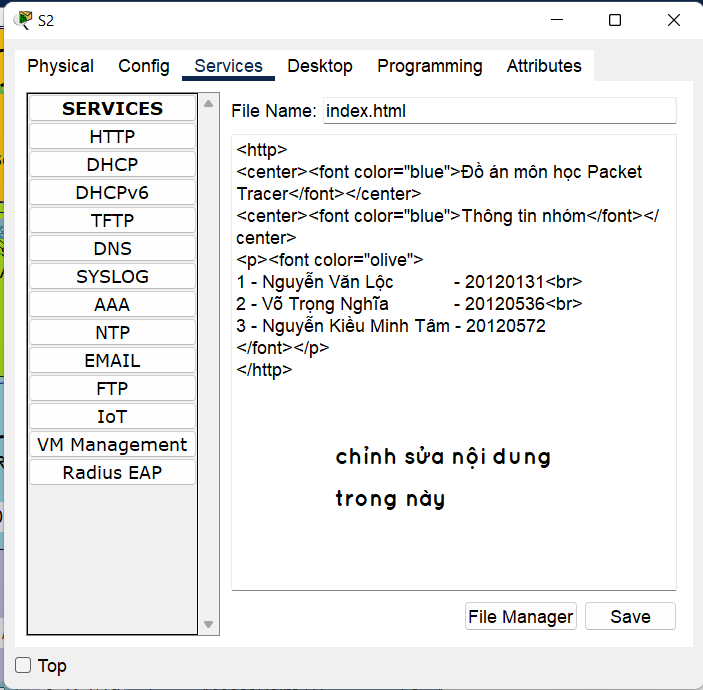
\includegraphics[scale=.7]{../figures/p2/web2}
\end{center}
\caption{Chỉnh sửa nội dung tập tin \texttt{\textcolor{blue}{index.html}}}
\end{figure}

Muốn truy cập trang web, vào tab Destop, chọn Web Browser và nhập www.mmt-72.com vào ô URL, màn hình sẽ hiện lên trang web. Các máy khác ở mạng khác muốn truy cập trang web này cũng làm tương tự, sau khi các subnet trong mô hình đã được kết nối với nhau hoàn tất.

\begin{figure}[H]
\begin{center}
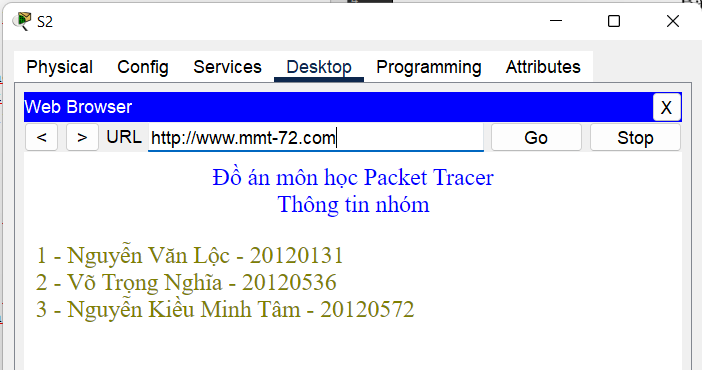
\includegraphics[scale=.7]{../figures/p2/web3}
\end{center}
\caption{Nội dung trang web \texttt{\textcolor{blue}{www.mmt-72.com}}}
\end{figure}

\item Định tuyến:

Ta thực hiện cấu hình các router R0, R1, R2.

Đối với router R0: 

+ Cổng Fa0/0 nối với subnet \texttt{\textcolor{blue}{172.72.0.0/19}} với địa chỉ IP \texttt{\textcolor{blue}{172.72.0.1/19}}, 

+ Cổng Fa1/0 nối với subnet \texttt{\textcolor{blue}{172.72.32.0/19}} với địa chỉ IP \texttt{\textcolor{blue}{172.72.32.1/19}}, 

+ Cổng Se2/0 nối với Se3/0 của R1 với địa chỉ IP \texttt{\textcolor{blue}{172.72.201.1/24}}, 

+ Cổng Se3/0 nối với Se2/0 của R2 với địa chỉ IP \texttt{\textcolor{blue}{172.72.202.2/24}}.

\begin{figure}[H]
\begin{center}
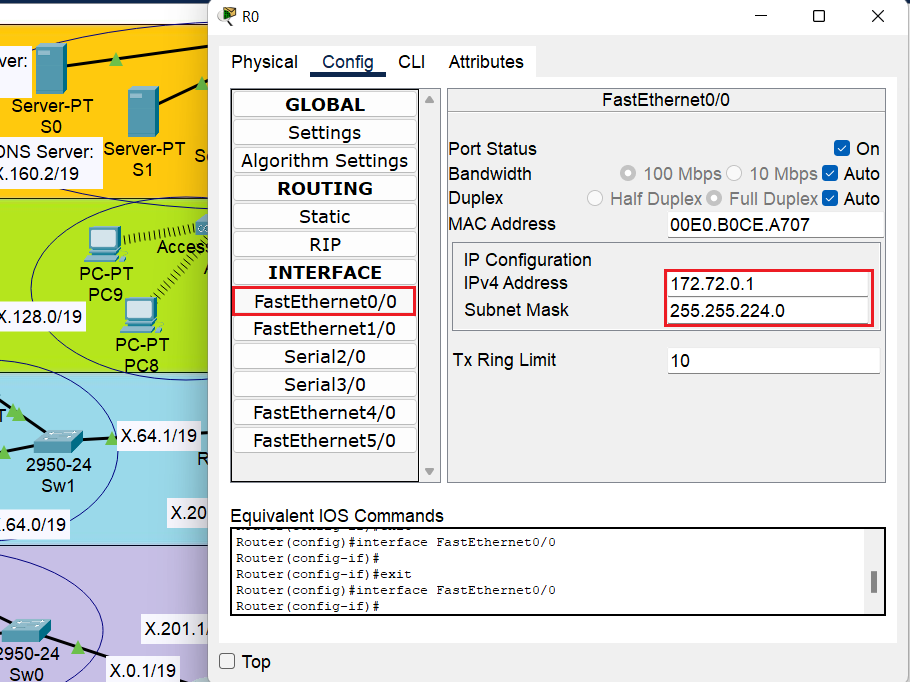
\includegraphics[scale=.7]{../figures/p2/routing1}
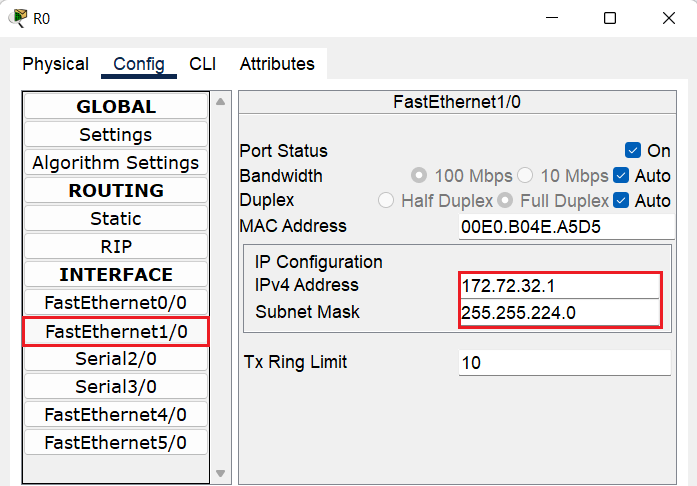
\includegraphics[scale=.6]{../figures/p2/routing2}
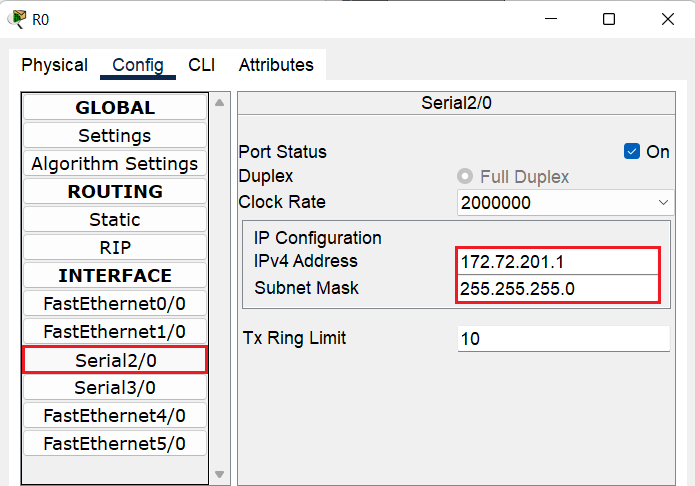
\includegraphics[scale=.6]{../figures/p2/routing3}
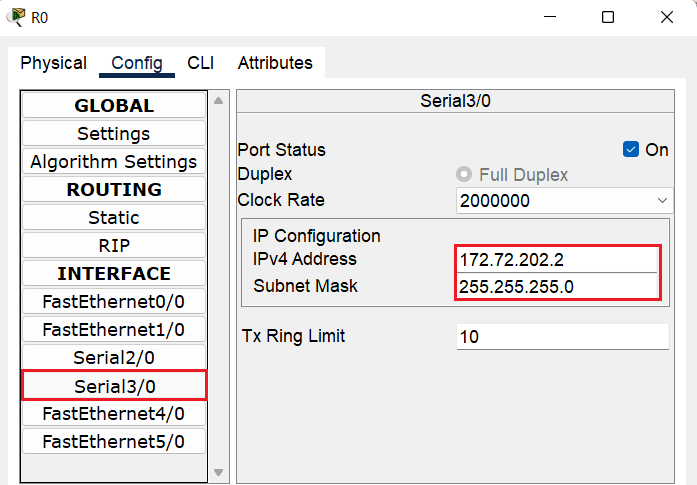
\includegraphics[scale=.6]{../figures/p2/routing4}
\end{center}
\caption{Cấu hình router R0}
\end{figure}

Ta thực hiện tương tự cho các router R1, R2 với các thông tin sau:

Đối với router R1: 

+ Cổng Fa0/0 nối với subnet \texttt{\textcolor{blue}{172.72.64.0/19}} với địa chỉ IP \texttt{\textcolor{blue}{172.72.64.1/19}}, 

+ Cổng Fa1/0 nối với subnet \texttt{\textcolor{blue}{172.72.96.0/19}} với địa chỉ IP \texttt{\textcolor{blue}{172.72.96.1/19}}, 

+ Cổng Se2/0 nối với Se3/0 của R2 với địa chỉ IP \texttt{\textcolor{blue}{172.72.212.1/24}}, 

+ Cổng Se3/0 nối với Se2/0 của R0 với địa chỉ IP \texttt{\textcolor{blue}{172.72.201.2/24}}.

Đối với router R2: 

+ Cổng Fa0/0 nối với subnet \texttt{\textcolor{blue}{172.72.128.0/19}} với địa chỉ IP \texttt{\textcolor{blue}{172.72.128.1/19}}, 

+ Cổng Fa1/0 nối với subnet \texttt{\textcolor{blue}{172.72.160.0/19}} với địa chỉ IP \texttt{\textcolor{blue}{172.72.191.254/19}}, 

+ Cổng Se2/0 nối với Se3/0 của R0 với địa chỉ IP \texttt{\textcolor{blue}{172.72.202.1/24}}, 

+ Cổng Se3/0 nối với Se2/0 của R1 với địa chỉ IP \texttt{\textcolor{blue}{172.72.212.2/24}}.

\item Cấu hình Access Point và truy cập mạng Wifi cho các thiết bị (nhân viên + khách ở tầng 1 và phòng họp ở tầng 3)

\begin{figure}[H]
\begin{center}
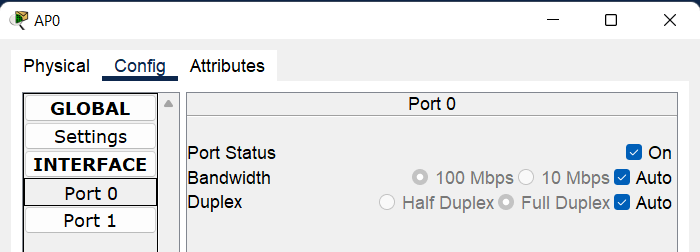
\includegraphics[scale=.6]{../figures/p2/ap1}
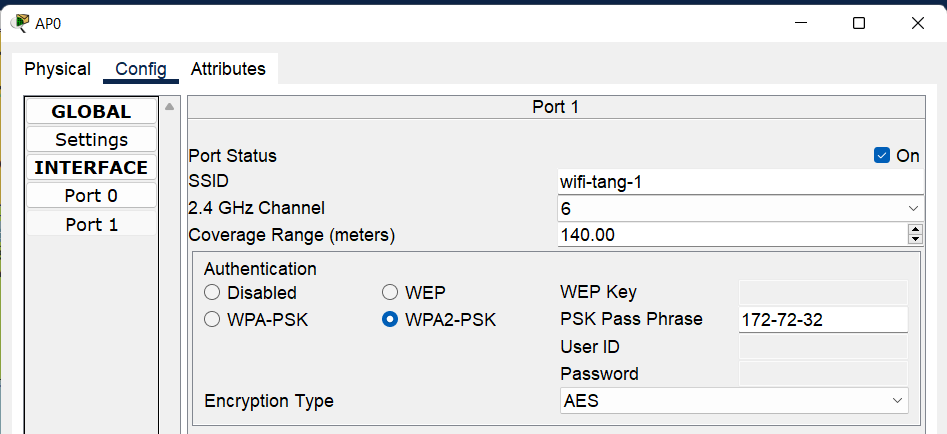
\includegraphics[scale=.6]{../figures/p2/ap2}
\end{center}
\caption{Cấu hình access point AP0 (nhân viên + khách vãng lai, tầng 1)}
\end{figure}

Thực hiện tương tự cho cấu hình access point AP1 cho phòng họp (tầng 3)
\begin{figure}[H]
\begin{center}
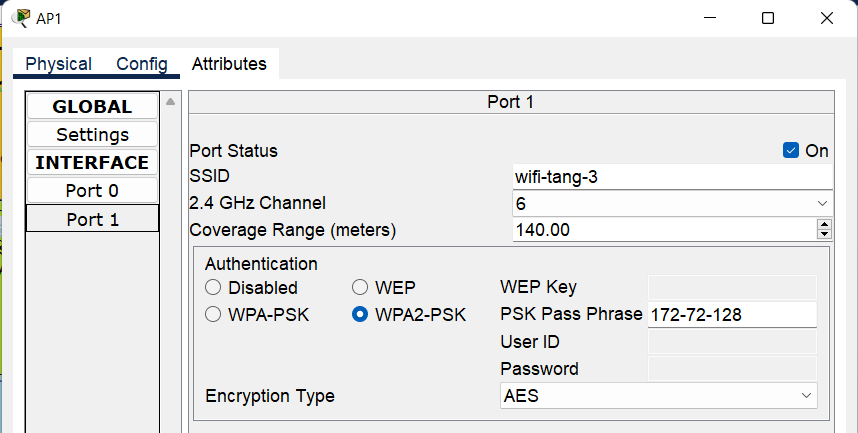
\includegraphics[scale=.6]{../figures/p2/ap3}
\end{center}
\caption{Cấu hình access point AP1, port 1}
\end{figure}

Để truy cập wi-fi, đối với PC/laptop, ta cần tắt chúng đi và thay thiết bị (PT-PC-NM-1CFE/PT-LAPTOP-NM-1CFE) bởi WMP300N/WPC300N, sau đó khởi động lại. Sau đó chuyển qua tab Destop, mở PC Wireless và thực hiện kết nối với mạng tương ứng.

\begin{figure}[H]
\begin{center}
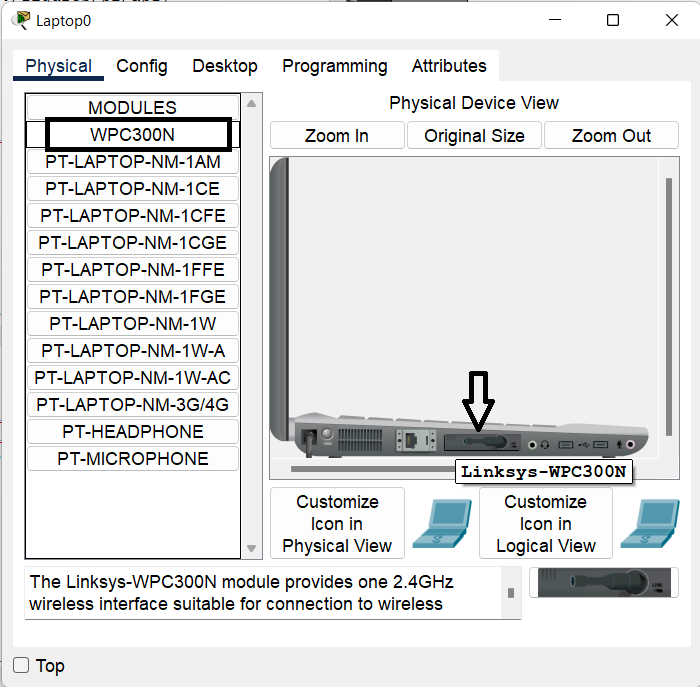
\includegraphics[scale=.6]{../figures/p2/ap4}
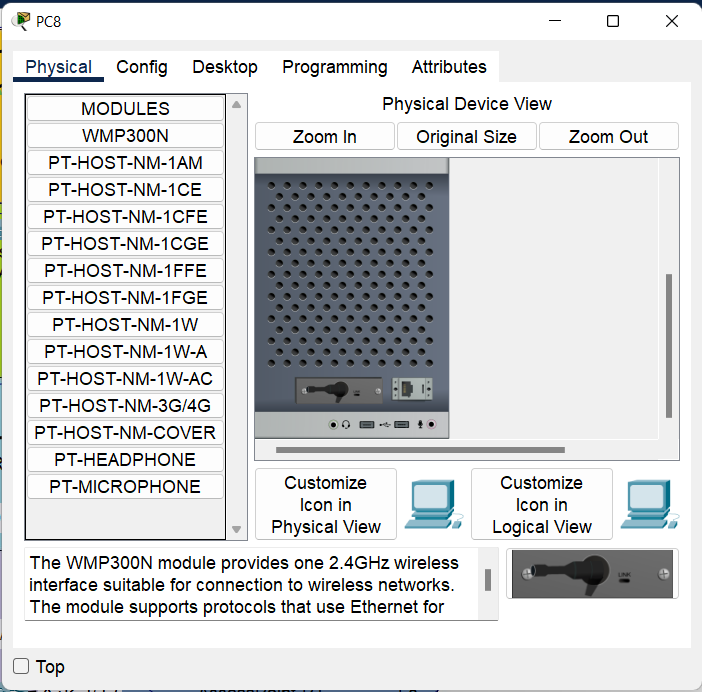
\includegraphics[scale=.6]{../figures/p2/ap9}
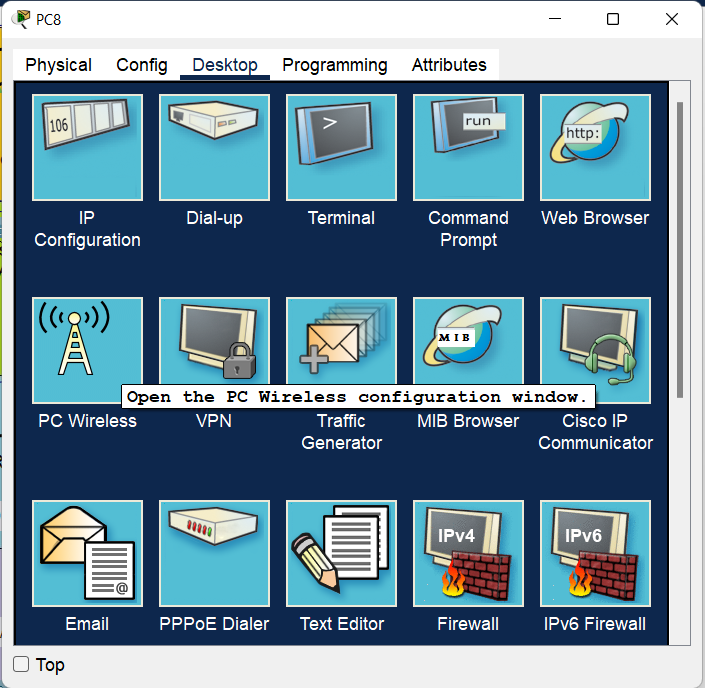
\includegraphics[scale=.5]{../figures/p2/ap5}
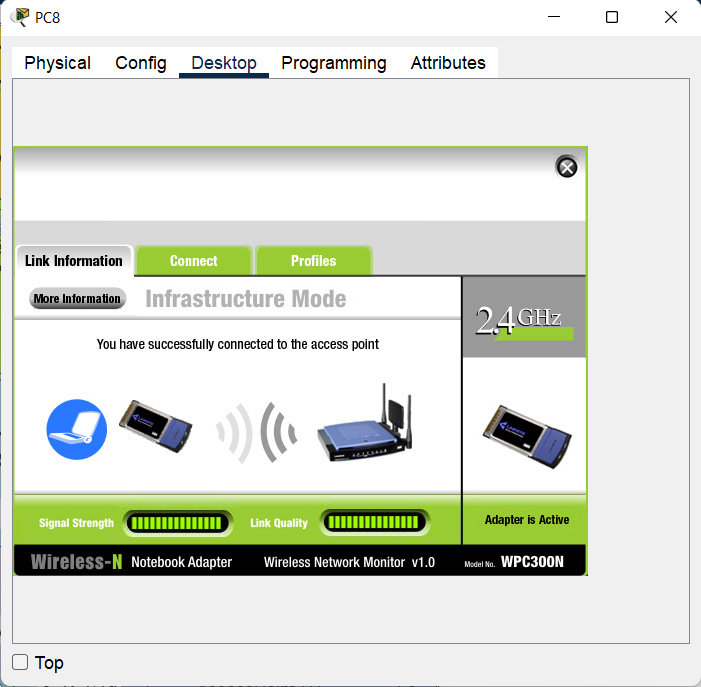
\includegraphics[scale=.5]{../figures/p2/ap6}
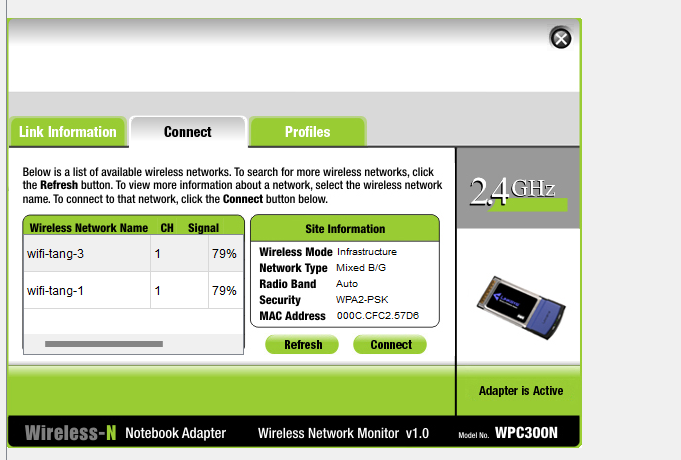
\includegraphics[scale=.6]{../figures/p2/ap7}
\end{center}
\caption{Kết nối từ PC/laptop đến wifi}
\end{figure}

Đối với điện thoại thông minh, ta vào tab Config và chọn thẻ Interface/Wireless0, sau đó nhập SSID, chọn Authenciation là WPA2-PSK và PSK Pass Phrase tương ứng với mạng cần kết nối.

\begin{figure}[H]
\begin{center}
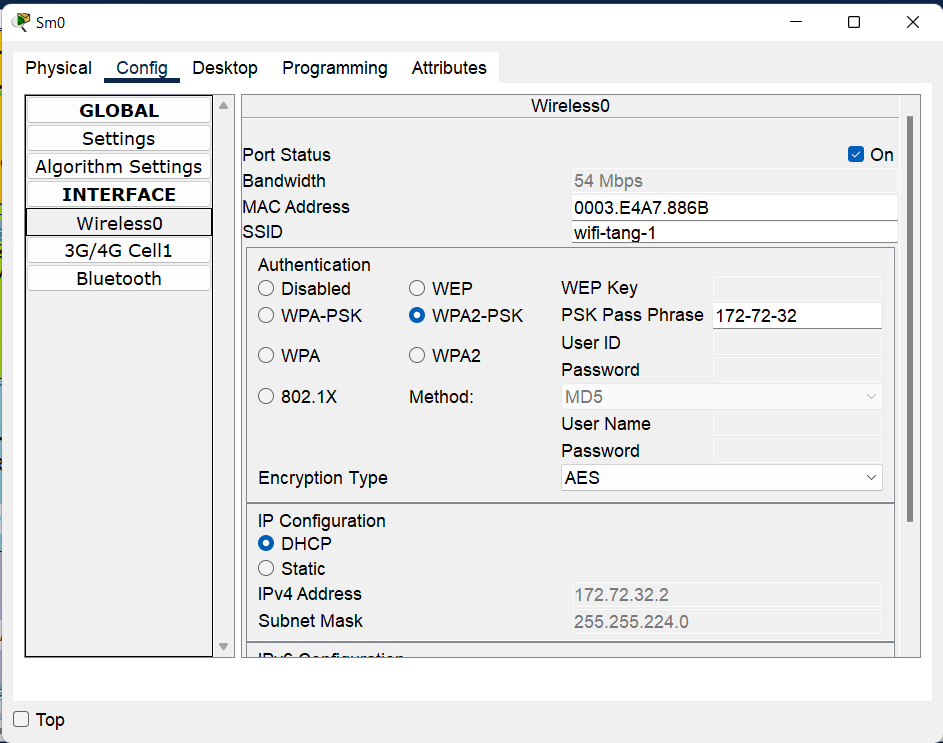
\includegraphics[scale=.6]{../figures/p2/ap10}
\end{center}
\caption{Kết nối từ smartphone đến wifi}
\end{figure}

\item Cấu hình IP tĩnh cho các server:

Mở server, vào tab Destop, chọn IP Configuration và sau đó nhập địa chỉ IP, subnet mask, default gateway và DNS server tương ứng (DNS server là 172.72.160.2, default gateway cho các server đều là 172.72.191.254, subnet mask là /19 hay 255.255.224.0)

\begin{figure}[H]
\begin{center}
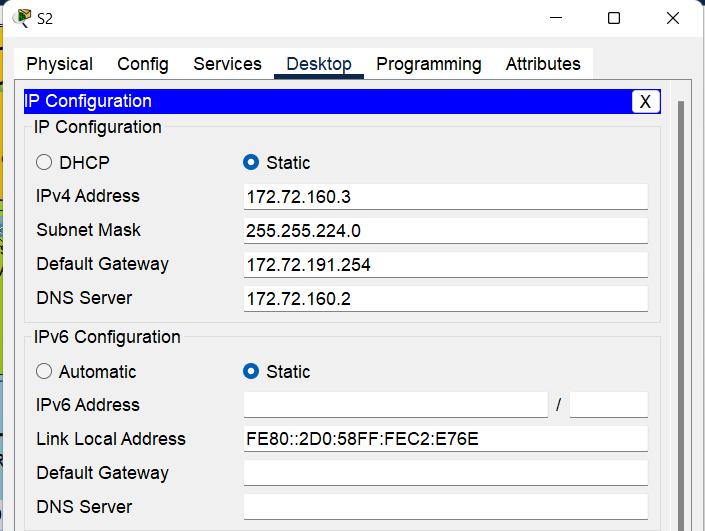
\includegraphics[scale=.6]{../figures/p2/ipconf}
\end{center}
\caption{Cấu hình địa chỉ IP tĩnh}
\end{figure}

\end{enumerate}
\bf \item Kiểm tra kết quả hoạt động của mô hình mạng vừa triển khai (dùng các câu lệnh console như ping, nslookup, ipconfig, và trình duyệt web)

\rm

\end{enumerate}








